\documentclass[10pt,a4paper,oneside]{article}
%\usepackage{blindtext}
\usepackage[utf8]{inputenc}
\usepackage[spanish,es-lcroman,es-nosectiondot,es-tabla]{babel}
%------------------------------------------------------
\usepackage{array,amssymb,amsthm,amsmath,amstext}
\usepackage{afterpage}% Necesario para introdicur páginas A3
\usepackage[font=scriptsize,bf]{caption}% Formato del caption
\usepackage{colortbl}% permite colorear tablas
\usepackage{booktabs} % To thicken table lines
\usepackage{longtable} % para tablas largas
\usepackage{eurosym}
\usepackage{emptypage}% evita la numeración de las páginas en blanco
\usepackage{fancyhdr,float}
\usepackage{graphicx}
\usepackage{listings} % premite la introducción de códigos vhdl
\usepackage{lscape}% Necesario para páginas apaisadas
\usepackage{mcode,multirow}
\usepackage{pdfpages}
\usepackage[paper=A4,pagesize]{typearea}%necesario para introducir páginas A3
\usepackage{setspace,subfigure}
\usepackage{titlesec}
\usepackage{xcolor}
\usepackage[colorlinks=true,linkcolor=udc,citecolor=udc]{hyperref}

% Fuente ----------------------------------------------------------
\usepackage{helvet}
\renewcommand*\familydefault{\sfdefault} 
%------------------------------------------------------------------
% Comandos personales
\definecolor{udc}{rgb}{0.81,0,0.49} % color de la UDC
\spanishdecimal{.} % escribe . en lugar de , para separar enteros de decimales
%\newcommand\crule[3][black]{\textcolor{#1}{\rule{#2}{#3}}}
\allowdisplaybreaks
%\renewcommand{\refname}{Referencias}
\newcommand{\IE}[3]{${}^{\scriptstyle^{#2}}_{\scriptstyle{\raisebox{-4pt}{}^{#3}}}{\text{#1}}$} % Elementos químicos

% Formato hoja----------------------------------------------
\renewcommand{\baselinestretch}{1.3}% interlineado
\headsep 15.5mm      \topmargin -2cm    \textheight 24.5cm     \textwidth 17cm    \oddsidemargin 0.04 cm   \evensidemargin -1.04cm
\footnotesep=20pt   \footskip=40pt
% Formato de las cabaceras de página -----------------------------------------------------------------
\usepackage{fancyhdr}
\pagestyle{fancy}
\fancyhf{} % borrar todos los ajustes
\fancyfoot[C]{\textbf{\scriptsize\thepage}}
% Modifica el ancho de las líneas de cabecera y pie
\renewcommand{\headrulewidth}{0pt}
%\renewcommand{\footrulewidth}{0.4pt}
\renewcommand{\footrule}{\hrule height 0.4pt \vspace{4mm}}
%%%%%%%%%%%%%%%%%%%%%%%%%%%%%%%%%%%%%%%%%%%%%%%%%%%%%%%%%%%%%%%%%%%%%%%%%%%%%%%%%%%%%%%%%%%%%%%%%%%%%%%%%%%%%%%%%%%%%%%%%%%%%%%%%%%
\usepackage{float}
\newfloat{Plano}{p}{pln}%[chapter]
\captionsetup[Plano]{labelformat=empty,labelsep=none,position=below}
%%%%%%%%%%%%%%%%%%%%%%%%%%%%%%%%%%%%%%%%%%%%%%%%%%%%%%%%%%%%%%%%%%%%%%%%%%%%%%%%%%%%%%%%%%%%%%%%%%%%%%%%%%%%%%%%%%%%%%%%%%%%%%%%%%%%
%--------------------------------------------------------------------
\setcounter{lofdepth}{2}% Introduce las subfiguras en lof
\allowdisplaybreaks
%%%%%%%%%%%%%%%%%%%%%%%%%%%%%%%%%%%%%%%%%%%%%%%%%%%%%%%%%%%%%%%%%%%%%%%%%%%%%%%%%%%%%%%%%%%
% Incluye la bibliografía como sección
%\makeatletter
%\renewenvironment{thebibliography}[1]
     %{\section{\refname}% esta línea cambia la bibliografía a la categoría sección
      %\@mkboth{\MakeUppercase\bibname}{\MakeUppercase\bibname}
      %\list{\@biblabel{\@arabic\c@enumiv}}%
           %{\settowidth\labelwidth{\@biblabel{#1}}
            %\leftmargin\labelwidth
            %\advance\leftmargin\labelsep
            %\@openbib@code
            %\usecounter{enumiv}
            %\let\p@enumiv\@empty
            %\renewcommand\theenumiv{\@arabic\c@enumiv}}
      %\sloppy
      %\clubpenalty4000
      %\@clubpenalty \clubpenalty
      %\widowpenalty4000%
      %\sfcode`\.\@m}
     %{\def\@noitemerr
       %{\@latex@warning{Empty `thebibliography' environment}}
      %\endlist}
%\makeatother
%%%%%%%%%%%%%%%%%%%%%%%%%%%%%%%%%%%%%%%%%%%%%%%%%%%%%%%%%%%%%%%%%%%%%%%%%%%%%%%%%%%%%%%%%%%%%%%%%%%%%%%%%%%%%%%%%%%%%%%%%%%%%%%%%%%%%%
\renewcommand\thesection{\arabic{section}}

% Se cambio el nombre del caption para los códigos
\renewcommand\lstlistingname{Código}
%%%%%%%%%%%%%%%%%%%%%%%%%%%%%%%%%%%%%%%%%%%%%%%%%%%%%%%%%%%%%%%%%%%%%%%%%%%%%%%%%%%%%%%%%%%%%%%%%%%%%%%%%%%%%%%%%%%%%%%%%%%%%%%%%%
% Incluye la bibliografía como subsección
\makeatletter
\renewenvironment{thebibliography}[1]
     {\subsection{\bibname}% esta línea cambia la bibliografía a la categoría sección
      \@mkboth{\MakeUppercase\bibname}{\MakeUppercase\bibname}
      \list{\@biblabel{\@arabic\c@enumiv}}%
           {\settowidth\labelwidth{\@biblabel{#1}}
            \leftmargin\labelwidth
            \advance\leftmargin\labelsep
            \@openbib@code
            \usecounter{enumiv}
            \let\p@enumiv\@empty
            \renewcommand\theenumiv{\@arabic\c@enumiv}}
      \sloppy
      \clubpenalty4000
      \@clubpenalty \clubpenalty
      \widowpenalty4000%
      \sfcode`\.\@m}
     {\def\@noitemerr
       {\@latex@warning{Empty `thebibliography' environment}}
      \endlist}
\makeatother
% Contador para todas las referencias
\newcounter{contador}
%%%%%%%%%%%%%%%%%%%%%%%%%%%%%%%%%%%%%%%%%%%%%%%%%%%%
\lstset{literate=%
         {á}{{\'a}}1 {é}{{\'e}}1 {í}{{\'i}}1 {ó}{{\'o}}1  {ú}{{\'u}}1 {ñ}{{\~n}}1
         {Á}{{\'A}}1 {É}{{\'E}}1 {Í}{{\'I}}1 {Ó}{{\'O}}1 {Ú}{{\'U}}1}
%--------------------------------------------------------------------------------------------------
\begin{document}

% PORTADA %%%%%%%%%%%%%%%%%%%%%%%%%%%%%%%%%%%%%%%%%%%%%%%%%%%%%%%%%%%%%%%%%%%%%%%%%%%%%%%%%%%%%%%%%%
\pagestyle{empty}

\begin{center} 

\includegraphics[scale=0.4]{Imagenes/PCB_Brain_circuit.png} 
\end{center}

\large

\vspace{3cm}

\begin{center}
{\setlength\arrayrulewidth{2pt}
\begin{tabular}{r|p{9.8cm}}
\arrayrulecolor{udc}
\colorbox{udc}{\textcolor{white}{\bf TÍTULO}}      
&	DISEÑO Y CONSTRUCCION DE UNA PLACA DE DESARROLLO PARA EL MICROCONTROLADOR STM32F103C8T6  \\[2cm]
%\colorbox{udc}{\textcolor{white}{\bf GRADO}}       & Dual en Ingeñaría Eléctrica    \\[1cm]
\colorbox{udc}{\textcolor{white}{\bf GRADO}}       & Ingenería Electrónica Industrial y Automática    \\[1cm]
\colorbox{udc}{\textcolor{white}{\bf ASIGNATURA}}  & Nombre de la asignatura     \\[2cm]
\colorbox{udc}{\textcolor{white}{\bf ESTUDIANTE}}  &	Garcia Camoira Cristobal  \\[2cm]
%                                                  &	Apellido1 Apellido 2, Nombres  \\[2cm]
\colorbox{udc}{\textcolor{white}{FECHA}}       &	Octubre de 2020
\end{tabular}}
\end{center}
\normalsize
% FIN DE LA PORTADA %%%%%%%%%%%%%%%%%%%%%%%%%%%%%%%%%%%%%%%%%%%%%%%%%%%%%%%%%%%%%%%%%%%%%%%%%%%%%%%%%%%%%%%%%%%%%%%%%%%%%%%%%%%%% -----------------------------------------------------------------------------------------------------------------------------------
\cleardoublepage

% Índice de contenidos
\pagestyle{plain}
\renewcommand{\contentsname}{Índice}
{\hypersetup{hidelinks}\tableofcontents}

\cleardoublepage

% Página que contiene el índice de listas de figuras
\phantomsection
\renewcommand*\listfigurename{Listado de figuras}
\addcontentsline{toc}{section}{\listfigurename}
{\hypersetup{hidelinks}\listoffigures}
\addtocontents{lof}{\protect\thispagestyle{plain}}

% Página que contiene el índice de listas de tablas
%\cleardoublepage
\phantomsection
\renewcommand*\listtablename{Listado de tablas}
\addcontentsline{toc}{section}{\listtablename}
{\hypersetup{hidelinks}\listoftables}
\addtocontents{lot}{\protect\thispagestyle{plain}}


% Página que contiene el índice de listados de programación
\renewcommand\lstlistlistingname{Listado de códigos de programación}
\renewcommand\lstlistingname{Código}
%\cleardoublepage
\phantomsection
\addcontentsline{toc}{section}{\lstlistlistingname}
{\hypersetup{hidelinks}\lstlistoflistings}
{\protect\thispagestyle{plain}}

% Final del índice -----------------------------------------------------------------------------------------------------------------------------------

\cleardoublepage %-----------------------------------------------------------------------------------------------------

\pagestyle{fancy}

\addcontentsline{toc}{section}{Introducción}%--------------------------------------------------------------------------------
\section*{Introducción}

El presente proyecto tiene como objetivo la realización de un sistema de evaluación que nos permita el uso de diferentes periféricos así como el uso de diferentes tipos de comunicación con diversos dispositivos. 

\section*{Características técnicas}

Este sistema poseerá las siguientes salidas:

\begin{enumerate}
	\item Salida para comunicación UART
	\item Salida para comunicación IIC
	\item Salida PWM
\end{enumerate}

Y también las siguientes entradas:

\begin{enumerate}
	\item Entrada ADC
	\item Entrada JTAG para la programación del microcontrolador
	\item Entrada para una batería que usara el DS1302 para que no se vaya de hora
\end{enumerate}

Este sistema incorporara internamente un LCD de 20 caracteres x 4 lineas que se conectara a nuestro microcontrolador través del expansor de entradas/salidas IIC PCF8574, ademas incorpora un DS1302, un reloj en tiempo real el cual se ha pensado manejar con el sistema de conexión 1 wire (conexión experimental), para el cual intentaremos usar el periférico interno USART.Todo esto nos permitirá el desarrollo de drivers para el correcto manejo de los dispositivos internos que posee y aprender de ello. Ademas las salidas que tenemos disponibles nos servirán para manejar otro tipo de dispositivos, dado que tenemos salida PWM, IIC y UART y una entrada para un ADC.

El microcontrolador que se usara en el proyecto pertenece al fabricante ST microelectronics, concretamente es el STM32F103C8T6, que incorporaremos a nuestro sistema ya en una placa de evaluación comúnmente denominada por la red de internet como "`Blue pill"', de hecho, si descargamos las librerías adecuadas se puede usar el entrono de Arduino para su programación, como si de un Arduino se tratase.

La alimentación de este sistema se hará a través del conector micro USB del que dispone la placa de evaluación de ST, un cargador de teléfono móvil sera mas que suficiente, 5V 1A, el resto de componentes internos se nutrirán de la alimentación de 5V que proporciona la placa de evaluación de ST dado que usa un regulador interno para ello.

\vspace{0.5cm}

\section{Lista de materiales y presupuesto}

% Table generated by Excel2LaTeX from sheet 'BOM'
\begin{center}
\begin{longtable}{|l|l|l|l|l|}

%primera parte de la tabla
\rowcolor[rgb]{ .267,  .447,  .769} \textcolor[rgb]{ 1,  1,  1}{\textbf{Category}} & \textcolor[rgb]{ 1,  1,  1}{\textbf{Quantity}} & \textcolor[rgb]{ 1,  1,  1}{\textbf{References}} & \textcolor[rgb]{ 1,  1,  1}{\textbf{Value}} & \textcolor[rgb]{ 1,  1,  1}{\textbf{Unit Cost}} \\
\endfirsthead
%Continuación de la tabla \\
\rowcolor[rgb]{ .267,  .447,  .769} \textcolor[rgb]{ 1,  1,  1}{\textbf{Category}} & \textcolor[rgb]{ 1,  1,  1}{\textbf{Quantity}} & \textcolor[rgb]{ 1,  1,  1}{\textbf{References}} & \textcolor[rgb]{ 1,  1,  1}{\textbf{Value}} & \textcolor[rgb]{ 1,  1,  1}{\textbf{Unit Cost}} \\
\endhead

% ultima parte de la tabla por pagina
%\multicolumn{6}{c}{ \textit{Presupuesto de dispositivos}-(ver pag siguiente)}  \\ 
\caption[Lista de materiales]{Lista de materiales}
%Continua en la siguiente pagina \\
\endfoot

% ultima parte de la tabla
\caption[Lista de materiales]{Lista de materiales}\label{TABLA1}
\endlastfoot

\midrule
\rowcolor[rgb]{ .851,  .882,  .949} Capacitors & 2      & C1,C2  & 6pF    & \euro0,35 \\
\midrule
Capacitors & 1      & C3     & 1.0u   & \euro0,35 \\
\midrule
\rowcolor[rgb]{ .851,  .882,  .949} Capacitors & 2      & C4,C5  & 10n    & \euro0,35 \\
\midrule
Resistors & 1      & R1     & 1k     & \euro0,15 \\
\midrule
\rowcolor[rgb]{ .851,  .882,  .949} Resistors & 8      & R2,R3,R4,R6,R7,R8,R9,R10 & 10k    & \euro0,15 \\
\midrule
Resistors & 1      & R5     & 100R   & \euro0,15 \\
\midrule
\rowcolor[rgb]{ .851,  .882,  .949} Resistors & 1      & R11    & 100k   & \euro0,15 \\
\midrule
Resistors & 1      & R12    & 4k7    & \euro0,15 \\
\midrule
\rowcolor[rgb]{ .851,  .882,  .949} Integrated Circuits & 1      & U1     & STM32F103 & \euro3,50 \\
\midrule
Integrated Circuits & 1      & U2     & DS1302 & \euro2,50 \\
\midrule
\rowcolor[rgb]{ .851,  .882,  .949} Integrated Circuits & 1      & U3     & PCF8574 & \euro2,50 \\
\midrule
Transistors & 2      & Q1,Q2  & 2N7002 & \euro0,50 \\
\midrule
\rowcolor[rgb]{ .851,  .882,  .949} Miscellaneous & 3      & ADC,PWM,UART & CONN-SIL3 & \euro0,40 \\
\midrule
Miscellaneous & 1      & BAT1   & BATTERY & \euro2,00 \\
\midrule
\rowcolor[rgb]{ .851,  .882,  .949} Miscellaneous & 2      & IIC,JTAG & CONN-H4 & €0,40 \\
\midrule
Miscellaneous & 1      & L1     &        & \euro0,25 \\
\midrule
\rowcolor[rgb]{ .851,  .882,  .949} Miscellaneous & 1      & LCD\_20X4 & CONN-H16 & \euro4,00 \\
\midrule
Miscellaneous & 1      & RENC1  & ROTARY\_ENCODER1 & \euro2,50 \\
\midrule
\rowcolor[rgb]{ .851,  .882,  .949} Miscellaneous & 1      & X1     & CRYSTAL & \euro0,50 \\
\bottomrule

\end{longtable}
\end{center}

% Table generated by Excel2LaTeX from sheet 'COSTE MATERIAL DE FABRICACION'
\begin{center}
\begin{longtable}{|lll|}

%primera parte de la tabla
\rowcolor[rgb]{ .267,  .447,  .769} \multicolumn{1}{|l|}{\textcolor[rgb]{ 1,  1,  1}{\textbf{Category}}} & \multicolumn{1}{l|}{\textcolor[rgb]{ 1,  1,  1}{\textbf{Quantity}}} & \textcolor[rgb]{ 1,  1,  1}{\textbf{Unit Cost}} \\
\endfirsthead
%Continuación de la tabla \\
\rowcolor[rgb]{ .267,  .447,  .769} \multicolumn{1}{|l|}{\textcolor[rgb]{ 1,  1,  1}{\textbf{Category}}} & \multicolumn{1}{l|}{\textcolor[rgb]{ 1,  1,  1}{\textbf{Quantity}}} & \textcolor[rgb]{ 1,  1,  1}{\textbf{Unit Cost}} \\
\endhead

% ultima parte de la tabla por pagina
%\multicolumn{6}{c}{ \textit{Presupuesto de dispositivos}-(ver pag siguiente)}  \\ 
\hline
\caption[Presupuesto]{Presupuesto}
%Continua en la siguiente pagina \\
\endfoot

% ultima parte de la tabla
\hline
\caption[Presupuesto]{Presupuesto }\label{TABLA2}
\endlastfoot

\midrule
\rowcolor[rgb]{ .851,  .882,  .949} Capacitors & 5      & 1,75 \\
\midrule
Resistors & 12     & 1,8 \\
\midrule
\rowcolor[rgb]{ .851,  .882,  .949} Integrated Circuits & 3      & 8,5 \\
\midrule
Transistors & 2      & 1 \\
\midrule
\rowcolor[rgb]{ .851,  .882,  .949} Miscellaneous & 10     & 11,25 \\
\midrule
\textbf{Total} & \textbf{32} & \textbf{24,3} \\

\end{longtable}
\end{center}

\section{Montaje}
\subsection{Guía de montaje}%------------------------------------------------------------------------------------------------------

El proceso de insolado no se explica en esta guía, con lo cual se explica el proceso de montaje una vez tenemos la PCB tras ese proceso y el proceso de taladrado de los agujeros. Se incluye como ejemplo la Figura (\ref{fig:001}).

\begin{figure}[H]
\centering
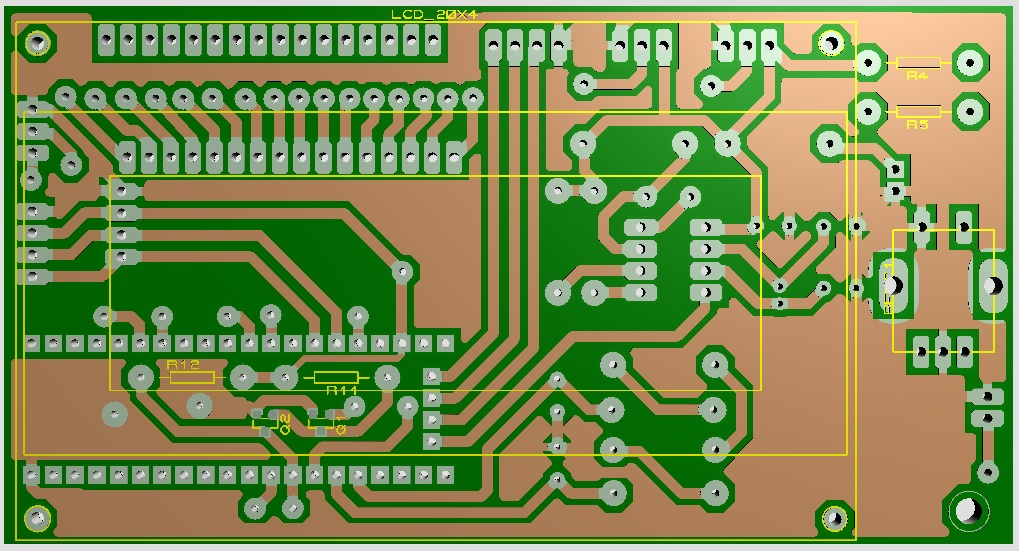
\includegraphics[scale=0.5]{Imagenes/PCB_CARA_DELANTERA.jpg}
\caption[Vista de las pistas de la cara delantera de la PCB tras el proceso de insolado]{Pistas PCB cara delantera}
\label{fig:001}
\end{figure}

\begin{figure}[H]
\centering
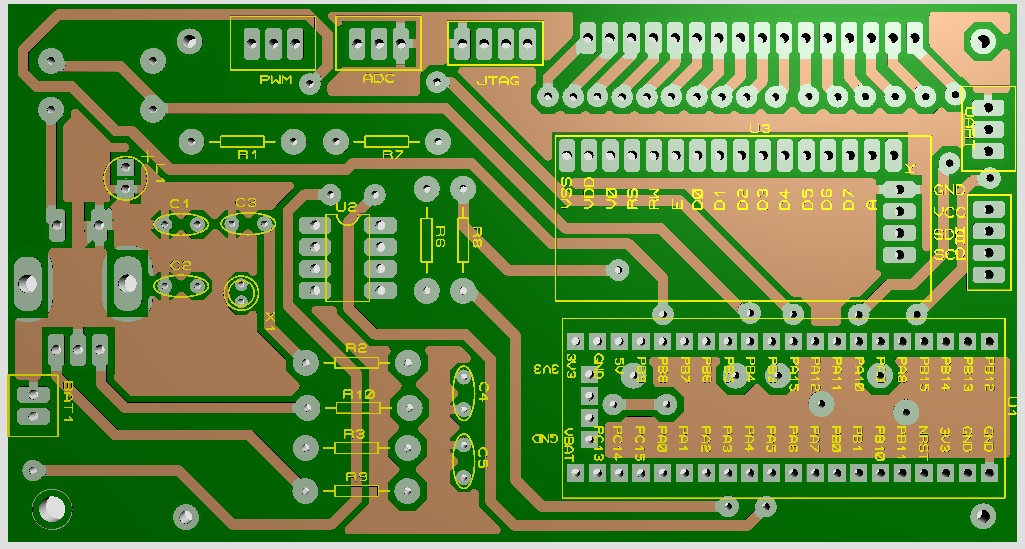
\includegraphics[scale=0.5]{Imagenes/PCB_CARA_TRASERA.jpg}
\caption[Vista de las pistas de la cara trasera de la PCB tras el proceso de insolado]{Pistas PCB cara trasera}
\label{fig:002}
\end{figure}

Teniendo como referencia la PCB por la cara delantera,  tal y como se representa en la imagen (\ref{fig:003}), los círculos señalados en rojo son las vías, es decir, los puntos que conectan ambas caras, delantera y trasera, esta conexión la haremos con unos cables rígidos que circularan de un lado al otro de la placa, soldados por ambas caras, para ello se puede usar un trozo de cable rígido pelado previamente. 

\begin{figure}[H]
\centering
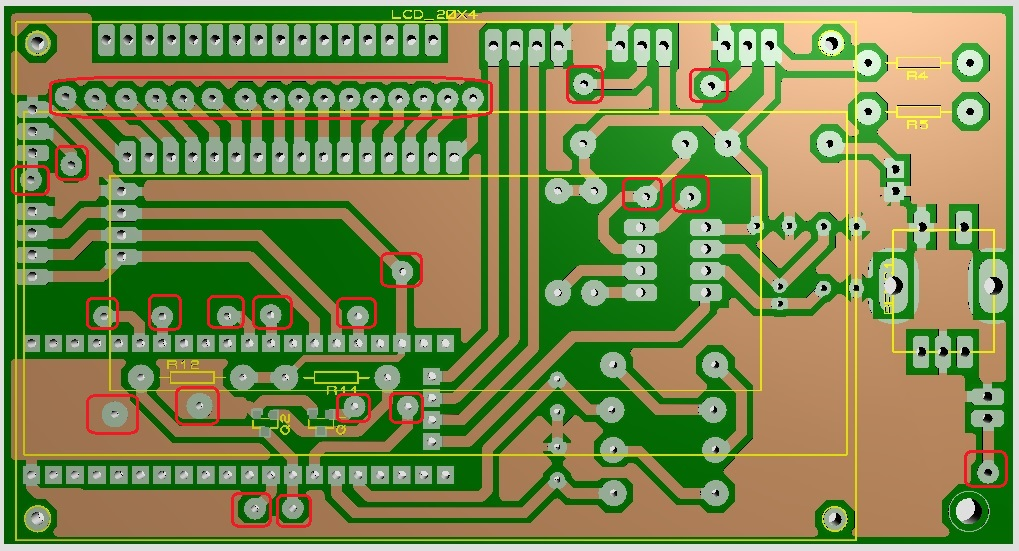
\includegraphics[scale=0.5]{Imagenes/PCB_CARA_DELANTERA_VIAS.jpg}
\caption[Vista de las vias de la cara delantera de la PCB tras el proceso de insolado]{Vías PCB cara delantera}
\label{fig:003}
\end{figure}

Una vez soldadas las vías, se recomienda ir soldando los componentes que vayan de menor a mayor volumen o tamaño para facilitar este proceso, Se recomienda empezar por soldar los que van por la parte trasera (\ref{fig:005}).
Por la cara delantera irán soldados los componentes: R4, R5, R11, R12, Q1, Q2, RENC1 y LCD20X4. En la imagen (\ref{fig:004}) no se pueden visualizar los componentes R11, R12, Q1 y Q2, dado que están justo debajo del LCD. El resto de componentes irán soldados por la parte trasera.

\begin{figure}[H]
\centering
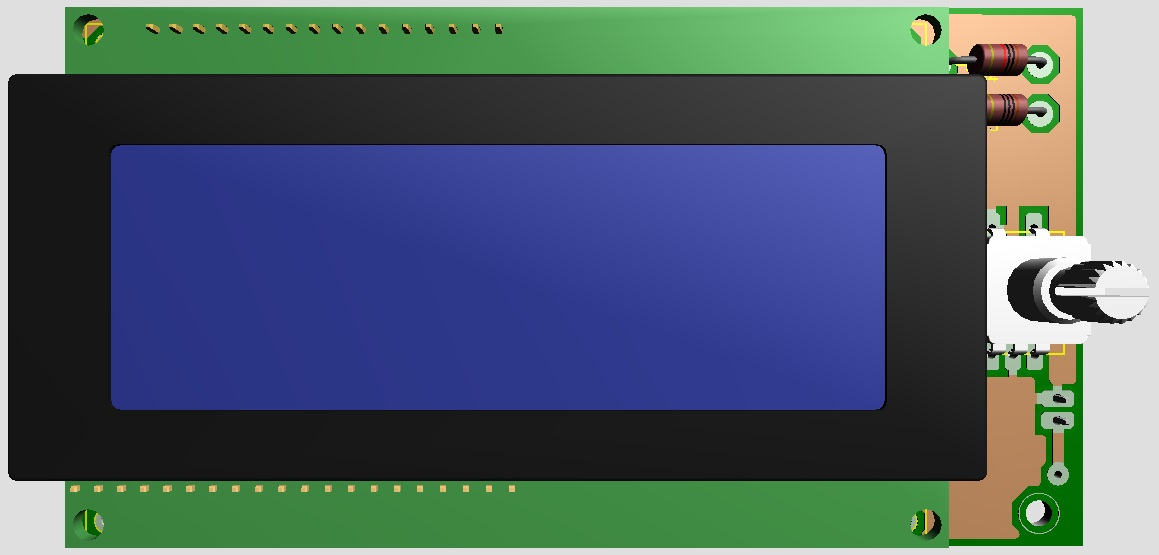
\includegraphics[scale=0.5]{Imagenes/PCB_COMPONENTES_CARA_DELANTERA.jpg}
\caption[Vista de los componentes de la cara delantera de la PCB]{Componentes de la cara delantera}
\label{fig:004}
\end{figure}

\begin{figure}[H]
\centering
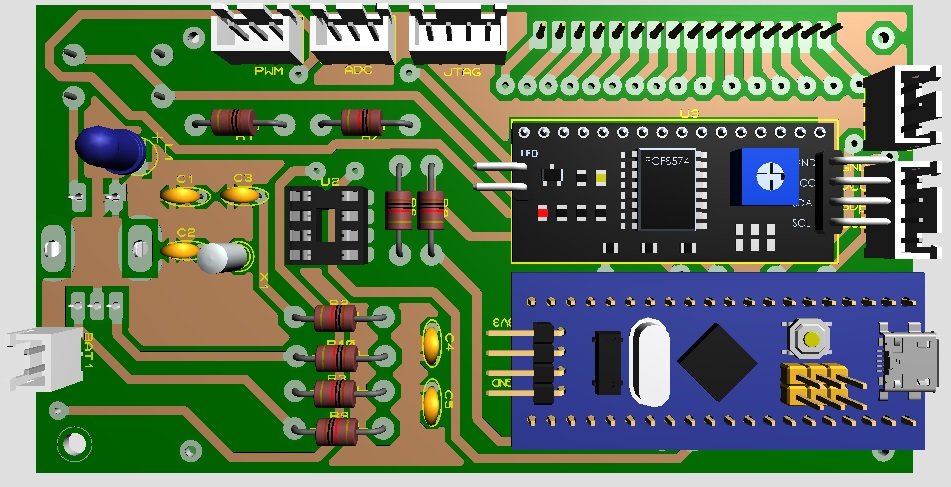
\includegraphics[scale=0.6]{Imagenes/PCB_COMPONENTES_CARA_TRASERA.jpg}
\caption[Vista de los componentes de la cara trasera de la PCB]{Componentes de la cara trasera}
\label{fig:005}
\end{figure}

\subsection{Programación del dispositivo}%------------------------------------------------------------------------------------------------------

Para la programación de este dispositivo se deben ejecutar los siguientes pasos:

\begin{enumerate}
	\item Conectar los pines del conector JTAG con sus homólogos en el programador stlink-V2.
	\item El código se encuentra en la siguiente dirección: \url{https://github.com/cristobalgc/STM32_PID_CONTROLLER}
	\item Esta sección se completara cuando el código este acabado.
\end{enumerate}

\section{Códigos de programación}%-------------------------------------------------------------------------------------------------

El código de programación del dispositivo estará localizado en el siguiente repositorio de github: \url{https://github.com/cristobalgc/STM32_PID_CONTROLLER}

\bigskip

\section{Sección Planos}%------------------------------------------------------------------------------------------------------

A continuación se introducen los planos. Cada plano figura en una página separada con numeración impar. La parte posterior de esas hojas deben estar en blanco.

%\pagestyle{fancy}


% FIN DE LA PORTADA
%%%%%%%%%%%%%%%%%%%%%%%%%%%%%%%%%%%%%%%%%%%%%%%%%%%%%%%%%%%%%%%%%%%%%%%%%%%%%%%%%%%%%%%%%%%%%%%%%%%%%%%%%%%%%%%%%%%%%%%%%%%%%%%%%%%%%%

% Principio Plano A4 ---------------------------------------------------------------------------------------------------
\cleardoublepage
\begin{Plano}[!htb]
\addcontentsline{toc}{subsection}{Esquema electrónico de la placa Blue pill} % Nombre que aparecerá en la lista de planos
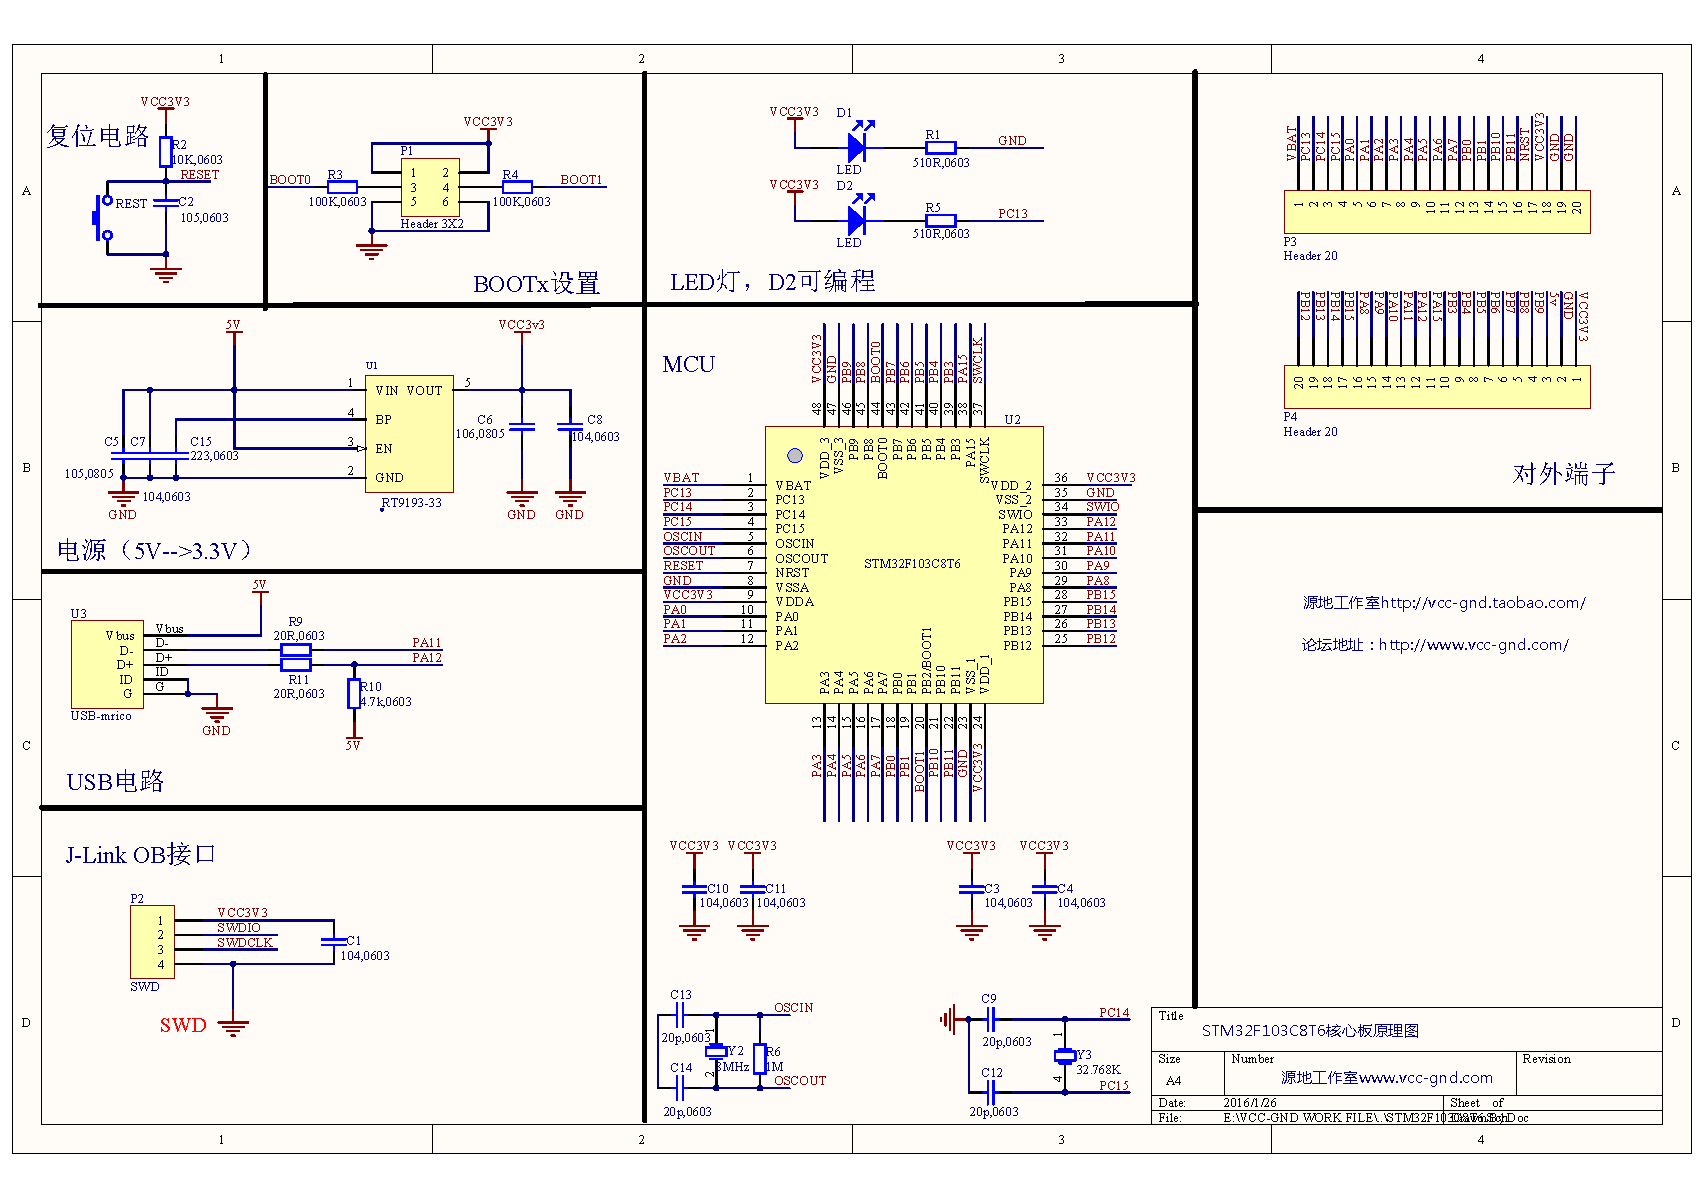
\includepdf[pages=-]{Planos/STM32F103C8T6-Blue_Pill-schematic.pdf} % Ruta y nombre del plano A4
\caption[Esquema electrónico de la placa Blue pill]{} % Página \thepage}
\label{BluePillSch} % Etiqueta para referenciar el plano
\end{Plano}

% Fin Plano A4 --------------------------------------------------------------------------------------------------------

% Principio Plano A4 ---------------------------------------------------------------------------------------------------
\cleardoublepage
\begin{Plano}[!htb]
\addcontentsline{toc}{subsection}{Esquema electrónico del expansor de entradas-salidas IIC} % Nombre que aparecerá en la lista de planos
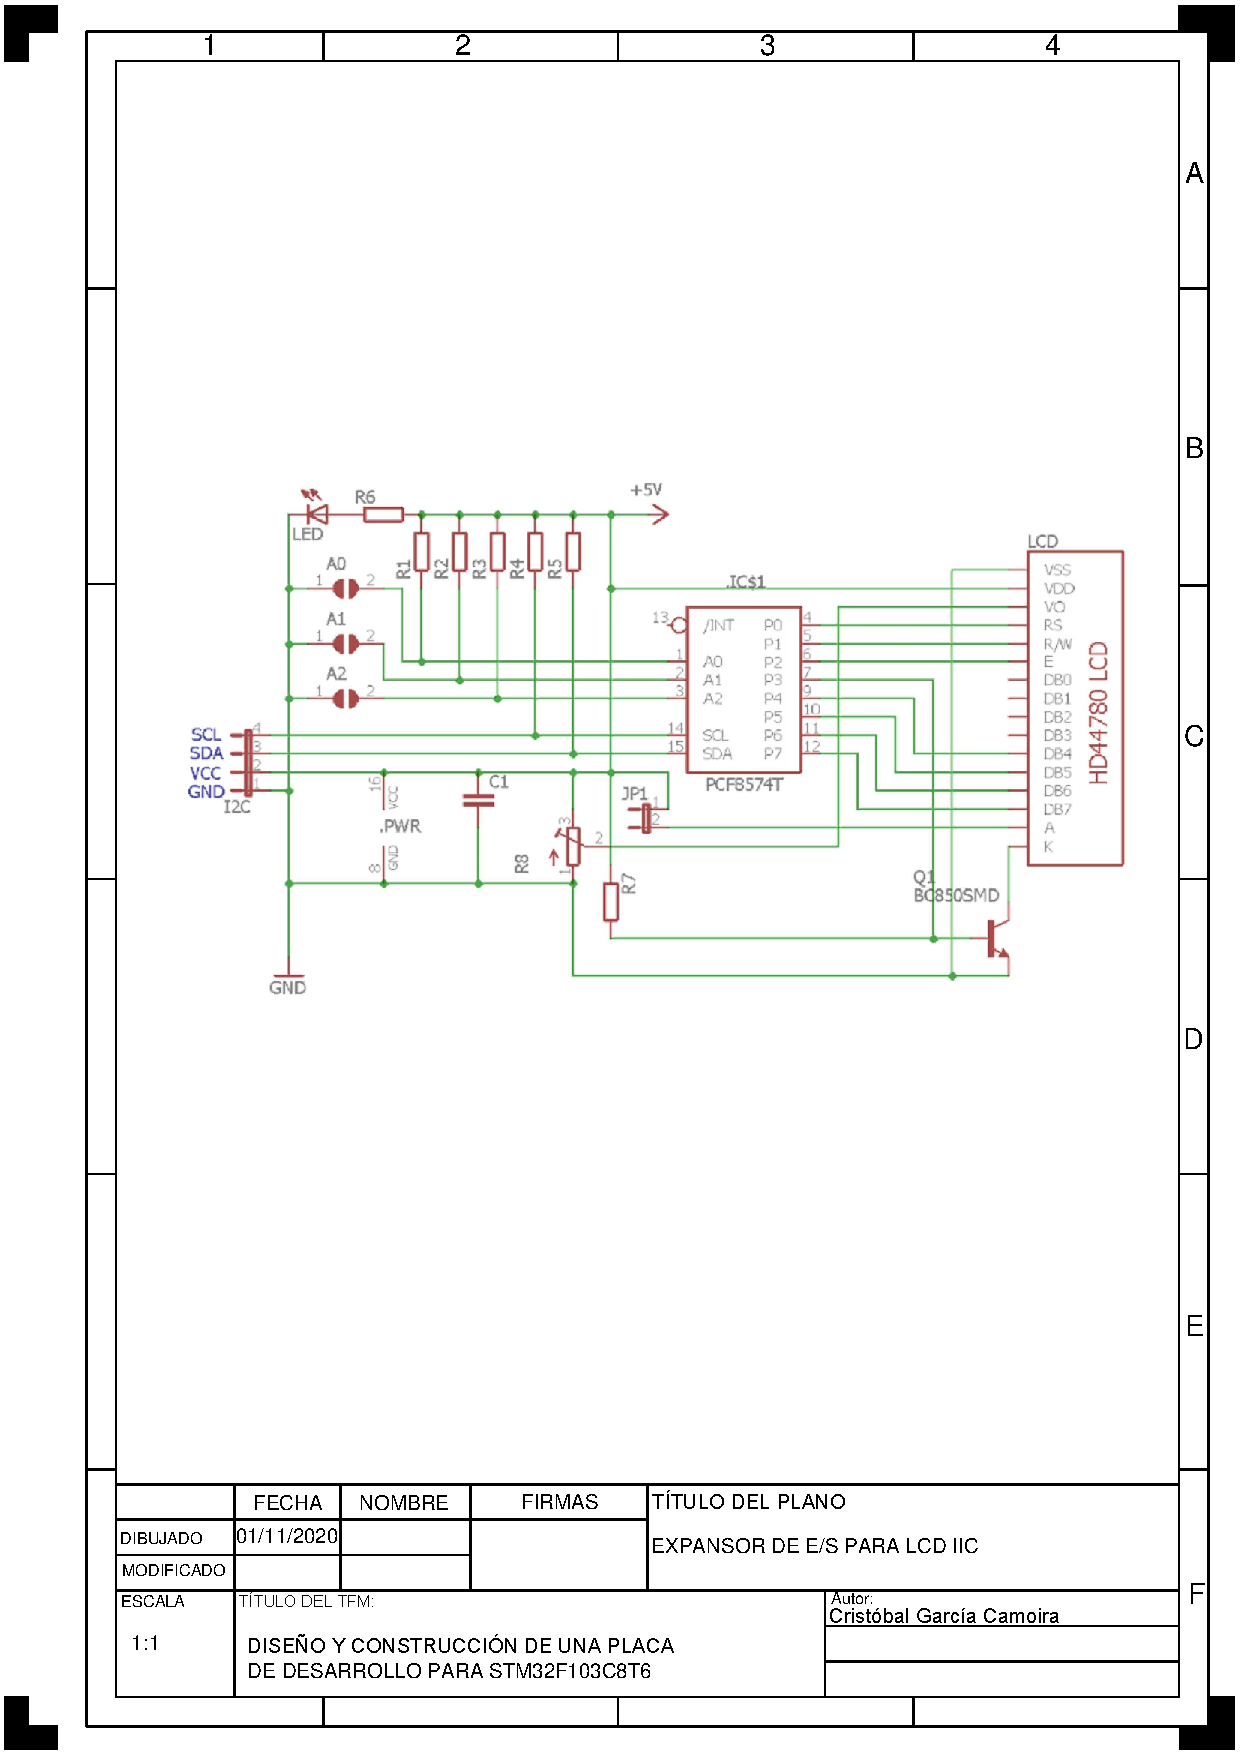
\includepdf[pages=-]{Planos/PCF8574_IO_Expander_schematic.pdf} % Ruta y nombre del plano A4
\caption[Esquema electrónico del expansor de entradas-salidas IIC]{} % Página \thepage}
\label{PCF8574Sch} % Etiqueta para referenciar el plano
\end{Plano}

% Fin Plano A4 --------------------------------------------------------------------------------------------------------


% Principio Plano A3 ---------------------------------------------------------------------------------------------------
\cleardoublepage

\begin{landscape} % se indica que empieza una página apaisada
\afterpage

\KOMAoptions{paper=A3,paper=landscape,pagesize}
\recalctypearea
\begin{Plano}[!htb]
\addcontentsline{toc}{subsection}{Placa de evaluación ST} % Nombre que aparecerá en la lista de planos
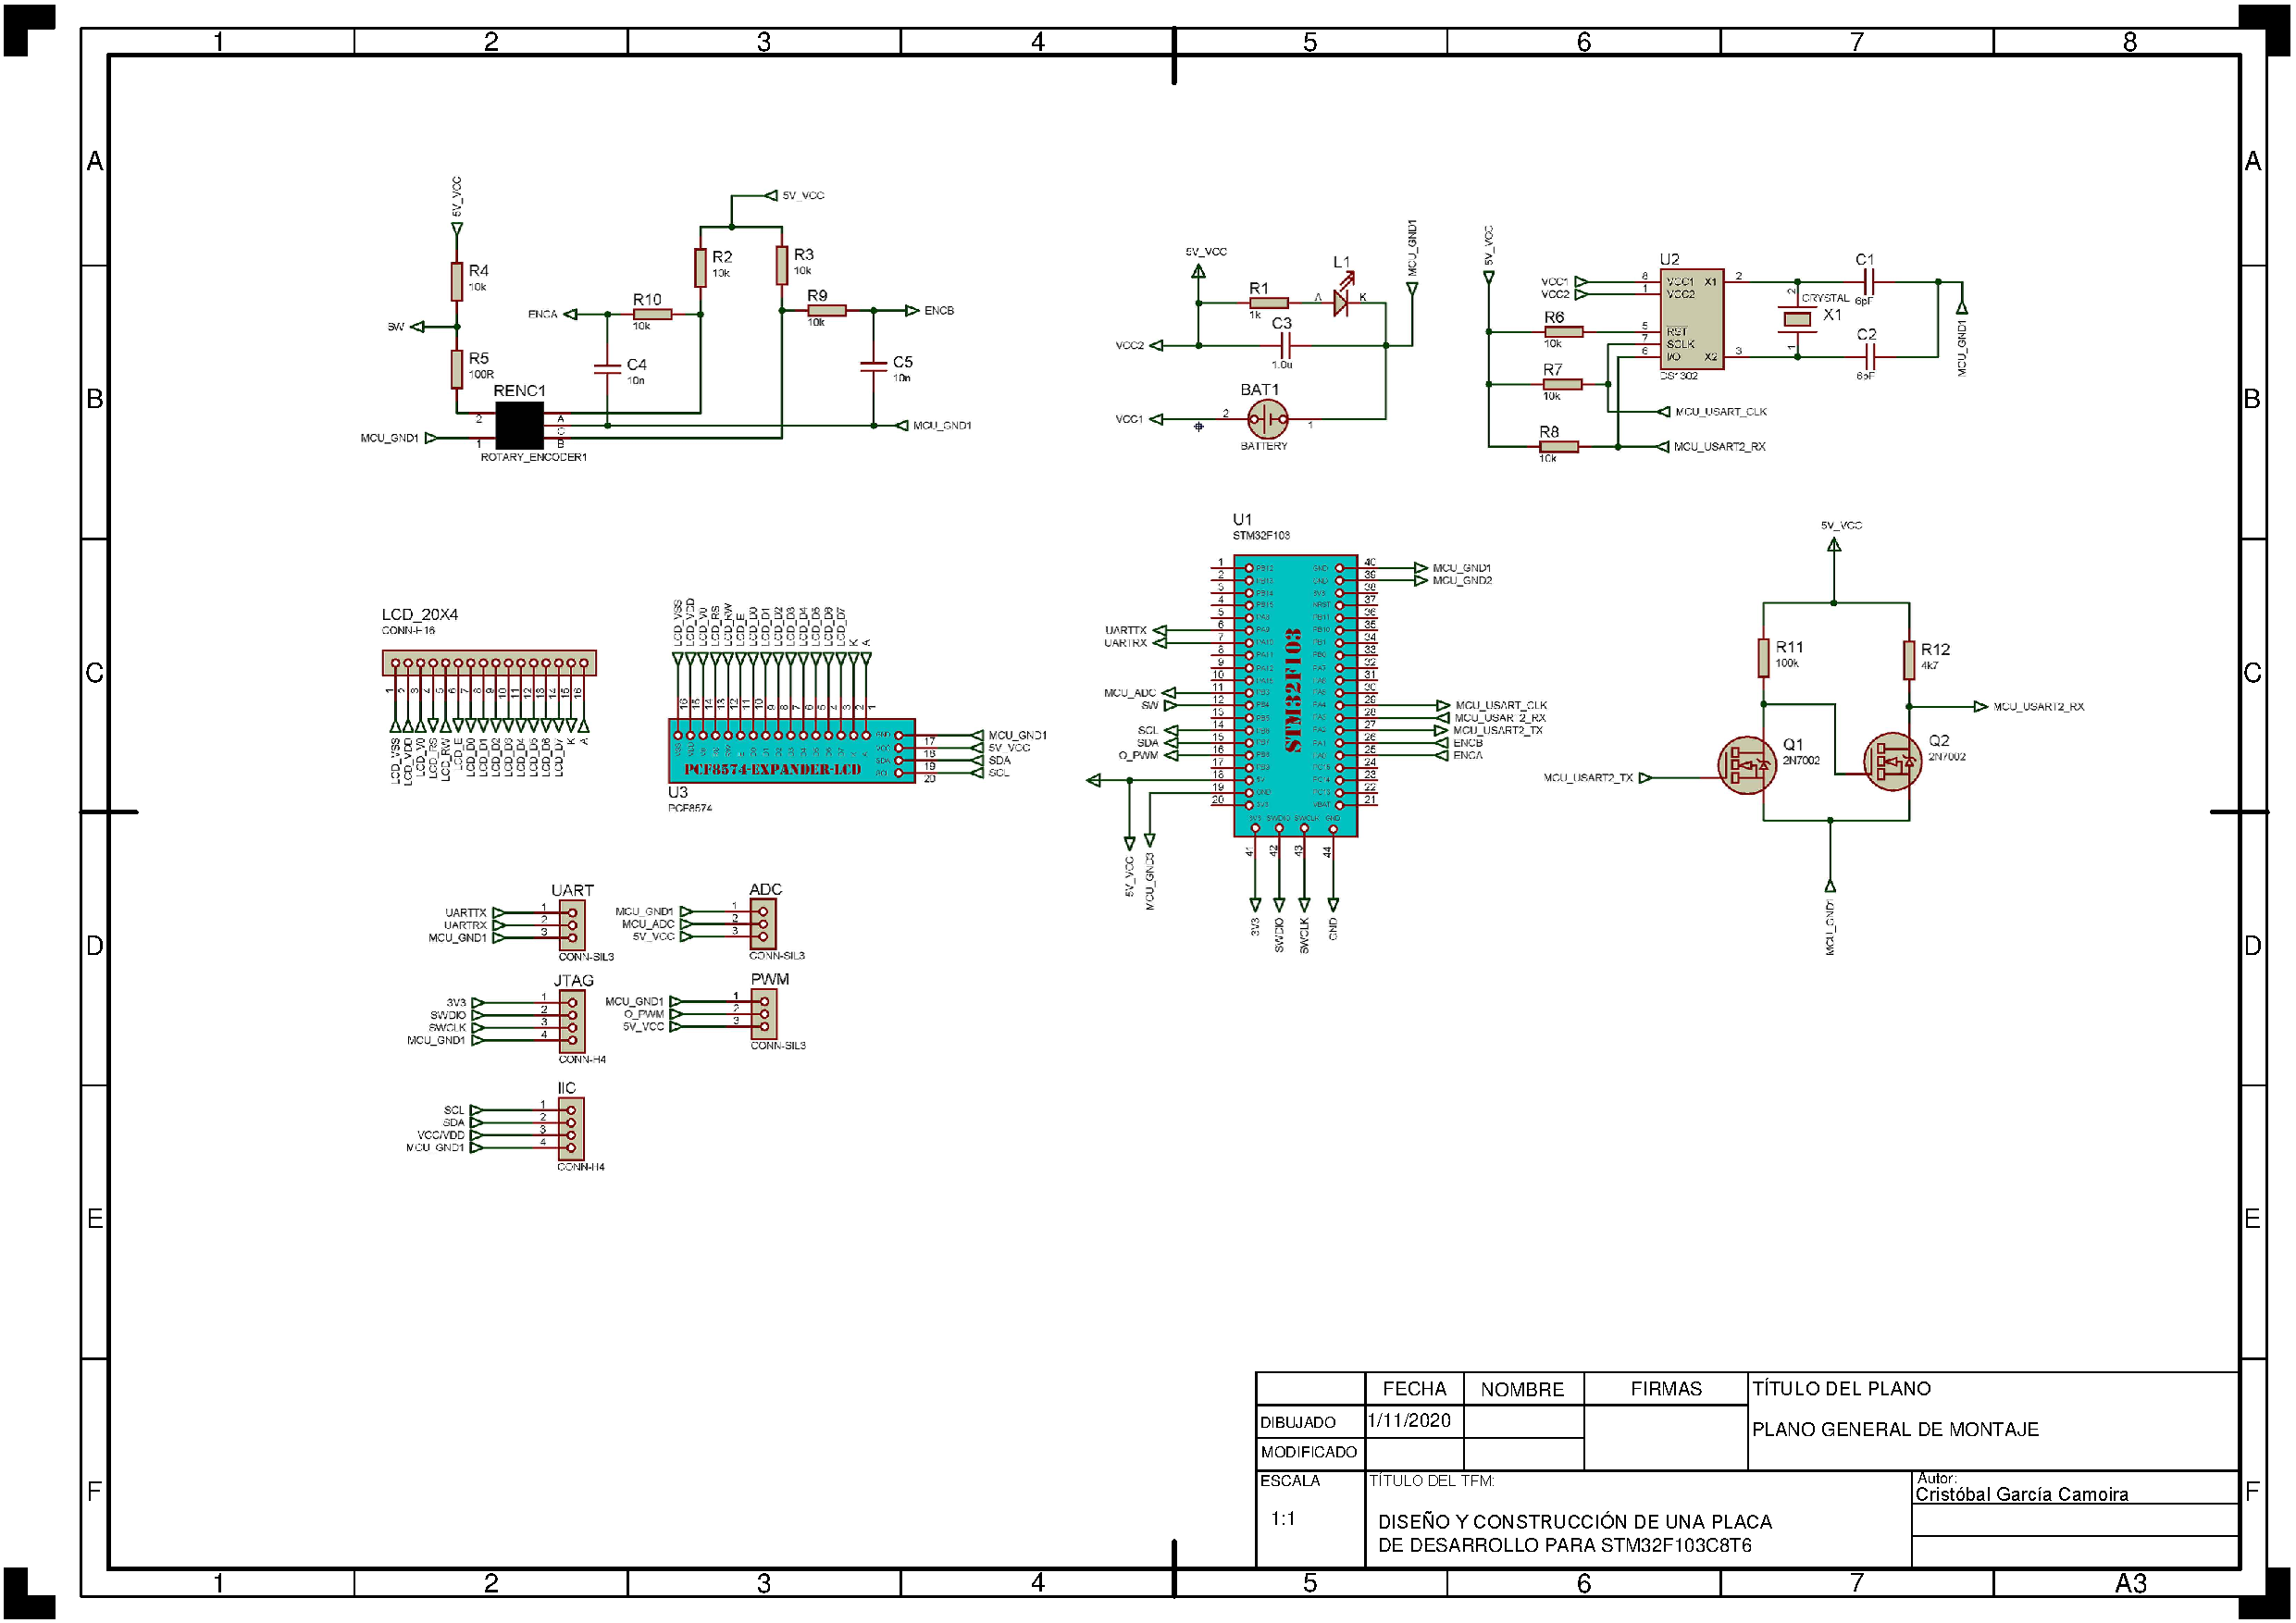
\includepdf[pages=-]{Planos/PCB_PLACA_EVAL_ST_SCHEMATIC.pdf} % Ruta y nombre del plano A3
\caption[Placa de evaluación ST]{}
\label{PacaEvalSch} % Etiqueta para referenciar el plano
\end{Plano}

\cleardoublepage

\KOMAoptions{paper=A4,pagesize}
\recalctypearea
\end{landscape} % se indica que acaba una página apaisada
% Fin Plano A3 --------------------------------------------------------------------------------------------------------

\cleardoublepage

% Principio Plano A4 ---------------------------------------------------------------------------------------------------
\cleardoublepage
\begin{Plano}[!htb]
\addcontentsline{toc}{subsection}{Fotolito PCB parte delantera} % Nombre que aparecerá en la lista de planos
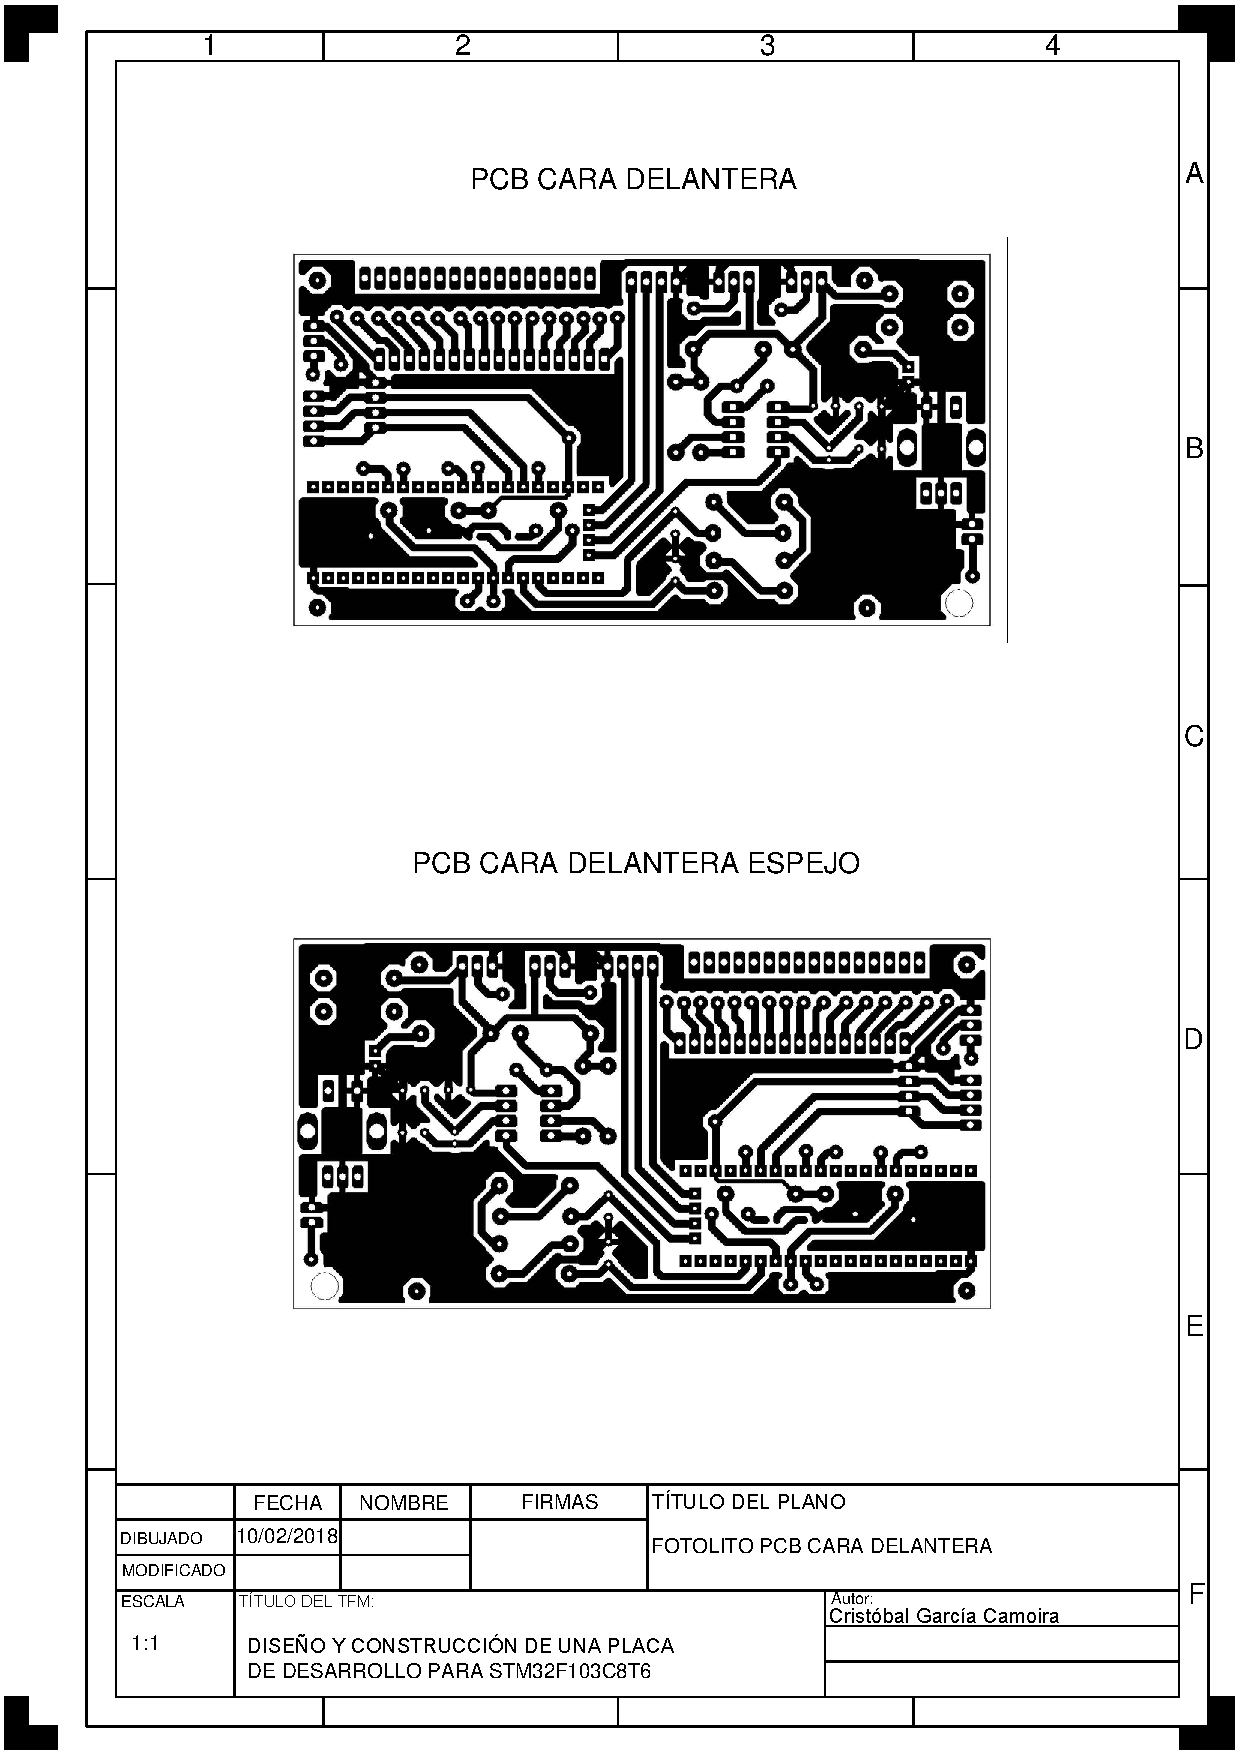
\includepdf[pages=-]{Planos/FOTOLITO_PCB_PARTE_DELANTERA.pdf} % Ruta y nombre del plano A4
\caption[Fotolito PCB parte delantera]{} % Página \thepage}
\label{FotolitoTOP} % Etiqueta para referenciar el plano
\end{Plano}

% Fin Plano A4 --------------------------------------------------------------------------------------------------------

% Principio Plano A4 ---------------------------------------------------------------------------------------------------
\cleardoublepage
\begin{Plano}[!htb]
\addcontentsline{toc}{subsection}{Fotolito PCB parte trasera} % Nombre que aparecerá en la lista de planos
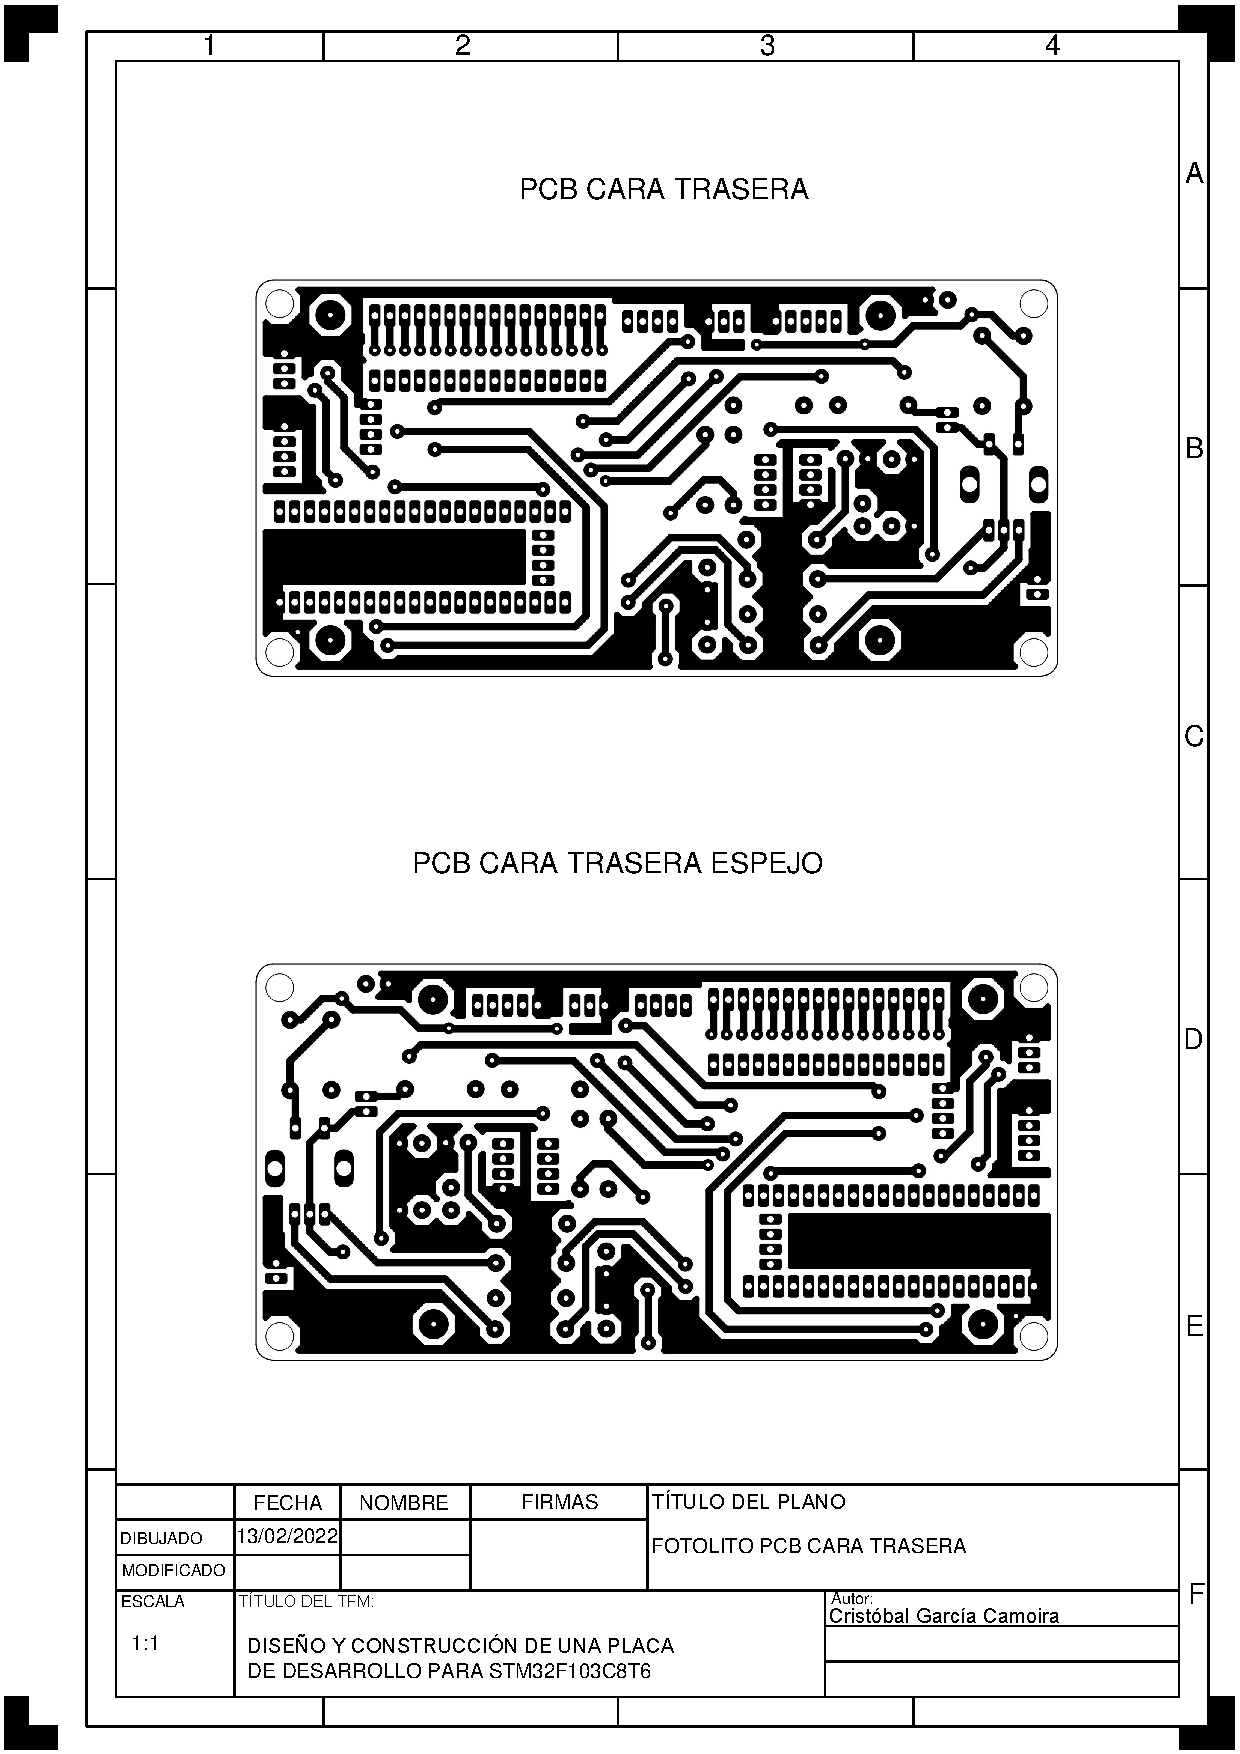
\includepdf[pages=-]{Planos/FOTOLITO_PCB_PARTE_TRASERA.pdf} % Ruta y nombre del plano A4
\caption[Fotolito PCB parte trasera]{} % Página \thepage}
\label{FotolitoBOT} % Etiqueta para referenciar el plano
\end{Plano}

% Fin Plano A4 --------------------------------------------------------------------------------------------------------

%%%%%%%%%%%%%%%%%%%%%%%%%%%%%%%%%%%%%%%%%%%%%%%%%%%%%%%%%%%%%%%%%%%%%%%%%%%%%%%%%%%%%%%%%%%%%%%%%%%%%%%%%%%%%%%%%%%%%%%%%%%%%%%%%%%%%%

\end{document}
